\documentclass[11pt,letterpaper]{article}
\usepackage[margin=0.62in,top=0.69in,bottom=0.66in,headheight=15pt,headsep=13pt,footskip=24pt]{geometry}
\usepackage{tikz,amsmath,amssymb,fancyhdr,array}
\usetikzlibrary{arrows.meta}
\usepackage[T1]{fontenc}\usepackage{lmodern}
\renewcommand{\familydefault}{\sfdefault}
\pagestyle{fancy}\fancyhf{}\fancyhead[L]{\small Week 72 / A robot that remembers / Grades 4--5}
\fancyfoot[L]{\scriptsize Bellingham Math Circle / Week 72 / GGT72-S-v1}\fancyfoot[R]{\scriptsize\thepage}
\renewcommand{\headrulewidth}{0.4pt}\renewcommand{\footrulewidth}{0pt}
\setlength{\parindent}{0pt}\setlength{\parskip}{8pt}
\newcommand{\problem}[2]{\textbf{Problem #1:} #2\par}
\newcommand{\grid}[5]{% minx maxx miny maxy scale
 \begin{tikzpicture}[scale=#5]
 \draw[step=1,gray!32,thin] (#1,#3) grid (#2,#4);
 \foreach \x in {#1,...,#2}{\node[below,font=\small] at (\x,#3) {\x};}
 \foreach \y in {#3,...,#4}{\node[left,font=\small] at (#1,\y) {\y};}
 \fill (0,0) circle (2.4pt); \node[above right,font=\small] at (0,0){O};
 \node[below,font=\small] at ({(#1+#2)/2},{#3-.48}) {column number};
 \end{tikzpicture}}
\newcommand{\lines}[1]{\foreach \n in {1,...,#1}{\noindent\rule{\linewidth}{0.2pt}\par\vspace{.24in}}}
\newcommand{\examplepanel}[3]{\begin{tikzpicture}[scale=.48]
 \draw[gray!30,step=1] (0,0) grid (3,1);
 \foreach \x in {0,1,2,3}{\node[below,font=\scriptsize] at (\x,0){\x};}
 \draw[-{Stealth[length=3pt]},line width=.8pt] #1;
 \fill #2 circle (3pt);
 \node[font=\small,anchor=north] at (1.5,-.8){#3};
 \end{tikzpicture}}
\begin{document}
Move one grid edge per card: E $\rightarrow$, W $\leftarrow$, N $\uparrow$, S $\downarrow$.
For N, add the column number to the memory. For S, subtract it.
E and W leave the memory unchanged.

One partner moves the robot; the other changes its memory marker and checks each move. Keep the cards in order so you can replay the route. Swap jobs for the next route. Each trial starts at the marked dot with memory 0.

\begin{center}
\begin{tabular}{c@{\quad}c@{\quad}c@{\quad}c}
\examplepanel{(0,0)--(0,0)}{(0,0)}{start: memory 0}&
\examplepanel{(0,0)--(2,0)}{(2,0)}{EE: memory 0}&
\examplepanel{(0,0)--(2,0)--(2,1)}{(2,1)}{EEN: memory 2}&
\examplepanel{(0,0)--(2,0)--(2,1)--(3,1)}{(3,1)}{EENE: memory 2}
\end{tabular}
\end{center}
\problem{1}{Use two E cards and two N cards, in any order. Find every different route from O to the ring. What memories can you leave there?}
\vspace{.05in}
\begin{minipage}[t]{.50\linewidth}\centering\vspace{0pt}
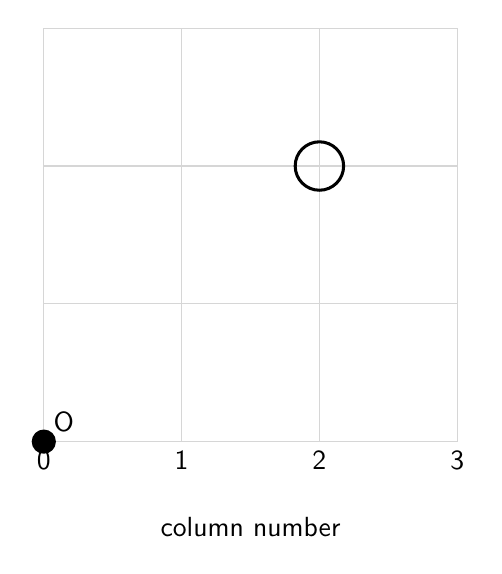
\begin{tikzpicture}[scale=1.75]
\draw[step=1,gray!32] (0,0) grid (3,3);
\foreach \x in {0,1,2,3}{\node[below] at (\x,0){\x};}
\fill (0,0) circle (2.5pt);\node[above right] at(0,0){O};
\draw[line width=1.1pt] (2,2) circle (5pt);
\node[below] at (1.5,-.48){column number};
\end{tikzpicture}
\end{minipage}\hfill
\begin{minipage}[t]{.43\linewidth}\vspace{0pt}
route\hfill final memory\par\vspace{.10in}
\lines{7}
\end{minipage}
\vfill
\begin{center}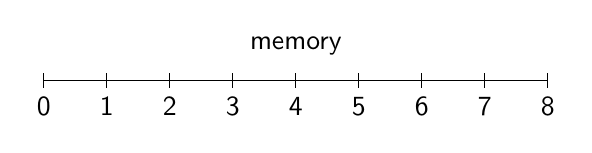
\begin{tikzpicture}[x=.8cm,y=.8cm]
\draw (0,0)--(8,0);\foreach \x in {0,...,8}{\draw(\x,-.12)--(\x,.12);\node[below]at(\x,-.12){\x};}\node[above]at(4,.25){memory};
\end{tikzpicture}\end{center}
\newpage
\problem{2}{Use E, N, W and S once each. Which memories can you leave when you return to O? Keep one route for each possible memory. Can any other memory occur with these four cards?}
\begin{center}\grid{-2}{2}{-2}{2}{2.15}\end{center}
\vspace{.1in}
\begin{center}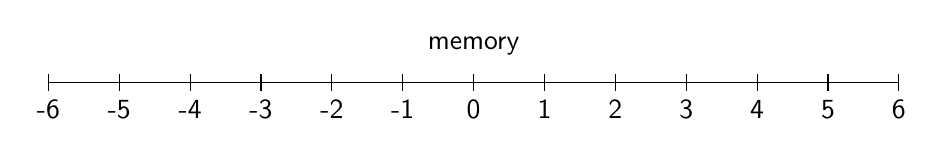
\begin{tikzpicture}[x=.9cm,y=.9cm]
\draw(-6,0)--(6,0);\foreach\x in{-6,...,6}{\draw(\x,-.12)--(\x,.12);\node[below]at(\x,-.12){\x};}\node[above]at(0,.25){memory};
\end{tikzpicture}\end{center}
\vspace{.1in}
route\hfill final memory\par\lines{3}
\vfill
\newpage
\problem{3}{Start at each dot with memory 0. Walk once around its outline in each direction. Write each memory beside an arrow showing your direction. How does moving the same rectangle to a new place affect its final memory? What connects a loop's shape, direction and final memory?}
\vspace{.1in}
\begin{center}
\begin{tabular}{c@{\hspace{.40in}}c}
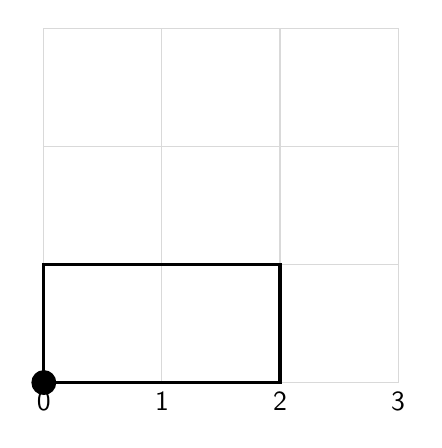
\begin{tikzpicture}[scale=1.50]
\draw[gray!30,step=1] (0,0) grid (3,3);\foreach\x in{0,...,3}{\node[below]at(\x,0){\x};}
\draw[very thick](0,0)--(2,0)--(2,1)--(0,1)--cycle;\fill(0,0)circle(3pt);
\end{tikzpicture}&
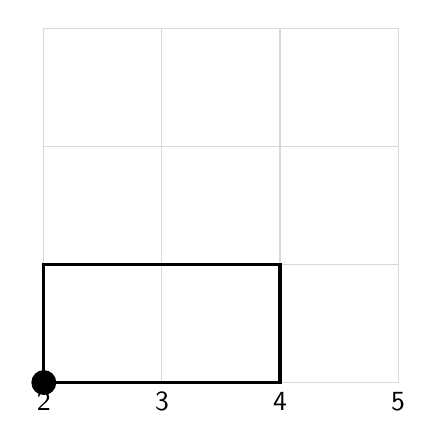
\begin{tikzpicture}[scale=1.50]
\draw[gray!30,step=1] (2,0) grid (5,3);\foreach\x in{2,...,5}{\node[below]at(\x,0){\x};}
\draw[very thick](2,0)--(4,0)--(4,1)--(2,1)--cycle;\fill(2,0)circle(3pt);
\end{tikzpicture}\\[5pt]
memories: \rule{.65in}{.3pt}, \rule{.65in}{.3pt}&memories: \rule{.65in}{.3pt}, \rule{.65in}{.3pt}\\[24pt]
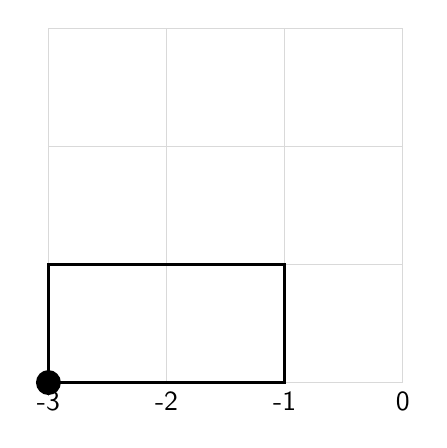
\begin{tikzpicture}[scale=1.50]
\draw[gray!30,step=1] (-3,0) grid (0,3);\foreach\x in{-3,...,0}{\node[below]at(\x,0){\x};}
\draw[very thick](-3,0)--(-1,0)--(-1,1)--(-3,1)--cycle;\fill(-3,0)circle(3pt);
\end{tikzpicture}&
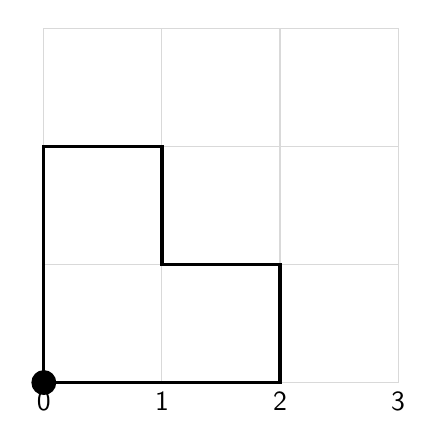
\begin{tikzpicture}[scale=1.50]
\draw[gray!30,step=1] (0,0) grid (3,3);\foreach\x in{0,...,3}{\node[below]at(\x,0){\x};}
\draw[very thick](0,0)--(2,0)--(2,1)--(1,1)--(1,2)--(0,2)--cycle;\fill(0,0)circle(3pt);
\end{tikzpicture}\\[5pt]
memories: \rule{.65in}{.3pt}, \rule{.65in}{.3pt}&memories: \rule{.65in}{.3pt}, \rule{.65in}{.3pt}
\end{tabular}\end{center}
\vspace{.12in}\lines{3}
\newpage
\problem{4}{Start at O with memory 0. Reach the ring with memory 7. Then start again and reach it with memory $-3$. You may use any number of E, N, W and S moves. Can you reach the ring with any whole-number memory, positive, zero or negative? Explain a plan.}
\begin{center}
\begin{tikzpicture}[scale=1.80]
\draw[gray!32,step=1] (-1,-1) grid (4,4);
\foreach\x in{-1,...,4}{\node[below]at(\x,-1){\x};}
\foreach\y in{-1,...,4}{\node[left]at(-1,\y){\y};}
\fill(0,0)circle(2.5pt);\node[above right]at(0,0){O};\draw[line width=1.1pt](2,2)circle(5pt);
\node[below]at(1.5,-1.48){column number};
\end{tikzpicture}
\end{center}
route to memory 7: \hrulefill\par\vspace{.17in}
route to memory $-3$: \hrulefill\par\vspace{.17in}
\lines{3}
\end{document}
